% DEFER-Dx: manuscript for JAMIA (Research and Applications). Build: bash paper/build.sh
% House style for this manuscript: no em dashes and no hyphens in running prose (numeric ranges are written
% "a to b"); hyphens remain only inside proper names (MIMIC-IV, Qwen3-8B, DEFER-Dx) and cited titles.
\documentclass[11pt]{article}
\usepackage[a4paper,margin=2.5cm]{geometry}
\usepackage{fontspec}
\setmainfont{texgyretermes}[Extension=.otf, UprightFont=*-regular, BoldFont=*-bold, ItalicFont=*-italic, BoldItalicFont=*-bolditalic]
\setsansfont{texgyreheros}[Extension=.otf, UprightFont=*-regular, BoldFont=*-bold, ItalicFont=*-italic, BoldItalicFont=*-bolditalic]
\usepackage{amsmath,amssymb}
\usepackage{graphicx}
\usepackage{booktabs,tabularx,multirow}
\usepackage{array}
\usepackage{xcolor}
\usepackage[font=small,labelfont=bf,labelsep=period,justification=raggedright,singlelinecheck=false]{caption}
\usepackage{setspace}
\usepackage{ragged2e}
\usepackage{cite}
\usepackage[hidelinks]{hyperref}
\usepackage{lineno}
\usepackage{float}

% no automatic hyphenation anywhere
\hyphenpenalty=10000 \exhyphenpenalty=10000 \sloppy
\newcommand{\act}[1]{\textsf{\textbf{#1}}}
\newcommand{\alttext}[1]{\par\smallskip{\RaggedRight\footnotesize\textit{Alt text:} #1\par}}
\newcolumntype{R}{>{\raggedleft\arraybackslash}X}
\newcolumntype{L}{>{\RaggedRight\arraybackslash}X}

\begin{document}
\RaggedRight
\setlength{\parindent}{1.5em}

% =========================== title page ===========================
\begin{titlepage}
\begin{center}
{\LARGE\bfseries Training clinical agents to ask, test, commit and defer:\\[4pt] a counterfactual reward for learned escalation to clinicians\par}
\vspace{1.2em}
{\large [Author names, degrees]\par}
\vspace{0.6em}
{[Department, institution, city, country for every author]\par}
\end{center}
\vspace{1.5em}
\noindent\textbf{Corresponding author:} [Full name, postal address, email, telephone]\\[6pt]
\textbf{Article type:} Research and Applications\\[6pt]
\textbf{Keywords:} Clinical Decision Support Systems; Reinforcement Learning; Large Language Models; Diagnosis; Referral and Consultation\\[6pt]
\textbf{Word count:} 3,137 (main text, excluding title page, abstract, references, figures and tables; \texttt{python3 paper/count\_words.py})\\[6pt]
\textbf{Code and benchmark:} \url{https://github.com/GIND123/Clinical-Agent-Stanford}
\end{titlepage}

% =========================== abstract ===========================
\section*{Abstract}
\noindent\textbf{Objective:} To train a diagnostic agent that learns when to hand a case to a clinician without collapsing into refusal, and to compare learned escalation with thresholding an identically trained agent.

\noindent\textbf{Materials and Methods:} DEFER-Dx, a Qwen3-8B agent trained by multiturn reinforcement learning, asks for the examination, orders any of 22 priced tests, commits to a diagnosis with a stated probability, or defers with a probabilistic differential. Each deferral is credited by a counterfactual escalation value: continuations branched from the deferral state, with deferral disabled, estimate the value of continuing. We evaluated 480 held out MIMIC-IV-Ext-CDM admissions, 393 admissions with other diagnoses, and 32 published case reports.

\noindent\textbf{Results:} DEFER-Dx answered 77.6\% of cases at 95.2\% accuracy (95\% CI 93.4 to 96.8), with 3.8 unflagged errors per 100 cases against 24.1 zero shot. Against the agent without deferral thresholded at matched coverage, it was more accurate on answered cases in all four seed pairings (pooled +3.2 points, 1.6 to 5.1). On 187 never seen time critical admissions, its two seeds committed wrongly in 6.8\% and 7.1\%, against 11.4\% for a published deferral reward. With clinicians modelled as following handoffs as often as physicians follow adversarial AI advice, team safety depended on the training seed.

\noindent\textbf{Discussion:} Crediting escalation against the counterfactual of continuing, within an escalation budget, gave stable, well targeted deferral; without the budget, the agent escalated almost everything.

\noindent\textbf{Conclusion:} Escalation can be learned; its safety depends on the handoff, which must be trained and evaluated against its reader.

\newpage
\linenumbers
\onehalfspacing

% =========================== background ===========================
\section*{Background and significance}

A patient arrives in the emergency department with abdominal pain. An interactive diagnostic agent asks for the examination, orders a CT and names a diagnosis. Every agent published on the MIMIC-IV clinical decision making benchmark (MIMIC-CDM)\cite{hager2024} must name one of four conditions (appendicitis, cholecystitis, diverticulitis or pancreatitis), even when the patient has a perforated ulcer or mesenteric ischaemia, and even when its own evidence is split. None can hand the case back.

Three developments make this gap pressing. First, regulators expect clinical decision support to leave the decision with a clinician who can independently review the basis of a recommendation\cite{fda2026}, and a randomised study of 225 physicians showed how fragile that safeguard is: conversational AI with a concealed objective raised harmful decisions from 2\% to 49\%, and expertise did not protect\cite{barrit2026}. Automation bias is a long standing concern of this journal's readership\cite{goddard2012}. Second, optimising accuracy alone has a cost: the strongest reported MIMIC-CDM agent reaches 93.4\% case weighted accuracy while its accuracy on the minority condition falls below that of a random test ordering policy\cite{ldtl}. Third, theory argues that an abstain action trained by reinforcement learning collapses into refusing everything, and that one should threshold a calibrated confidence after training instead\cite{che2026}.

Informatics work on abstention has taken that second route. Selective classifiers that abstain between two cost based thresholds and route the remaining cases to human abstractors improved clinical data extraction\cite{swaminathan2024}; sample consistency discriminates correct from incorrect language model diagnoses better than stated confidence, though calibration stays poor\cite{savage2025}; and an auditor that suppresses unreliable predictions improved simulated clinician and AI teams on MIMIC-IV-ED, but not when the clinician was the more accurate partner\cite{brown2026}. Learning to defer trains a rejector jointly with the predictor\cite{mozannar2020,madras2018,dvijotham2023}. Reinforcement learning rewards for deferral in language models price escalation by the policy's estimated case level success rate\cite{tiar,karl,awarl} or by designated cases\cite{trustmed}. None of these credits an escalation at the exact state where it happens in a multistep diagnostic episode, and none asks what the clinician who receives the case does with what the agent hands over.

\section*{Objective}

We asked three questions. Can an interactive agent learn when to defer without collapsing? Does learned deferral beat a confidence threshold on an identically trained agent at exactly matched coverage? And what happens once the case reaches a clinician who may follow the handoff? Our contributions are a reward, the counterfactual escalation value, that credits each escalation against what continuing from the same state would have achieved; two open world test sets, one of which can be shared without a data use agreement; and a head to head test of learned against post hoc deferral with two training seeds per arm and a model of the receiving clinician.

% =========================== methods ===========================
\section*{Materials and methods}

\subsection*{Data}
MIMIC-IV-Ext-CDM 1.1\cite{hager2024,johnson2023} contains 2,400 emergency admissions with acute abdominal pain (957 appendicitis, 648 cholecystitis, 538 pancreatitis, 257 diverticulitis). We kept the 80/10/10 split of LA-CDM\cite{lacdm} so that results are comparable on its test set. We built MIMIC-CDM-OW from MIMIC-IV 2.2: admissions with an abdominal chief complaint whose principal diagnosis falls in one of nine other groups, built with MIMIC-CDM's own text pipeline. It yields 713 OTHER cases and 648 same pipeline in set controls, which remove the shortcut ``built by the new pipeline, therefore OTHER''. Cohorts are patient disjoint (Table~\ref{tab:cohorts}; Supplementary Figure S1). Five time critical groups (mesenteric ischaemia, perforated or bleeding ulcer, ruptured aortic aneurysm, diabetic ketoacidosis, ectopic pregnancy) are held out of training entirely. MIMIC-CDM-CR contains 32 cases rebuilt from open access case reports published 2020 or later: 19 out of scope and 13 in scope, 9 of them complicated. Groups with fewer than 10 cases are reported only pooled.

\begin{table}[t]
\caption{Patient disjoint cohorts.}\label{tab:cohorts}
\small
\begin{tabularx}{\linewidth}{@{}lrL@{}}
\toprule
Cohort & Cases & Composition and use \\
\midrule
Reinforcement learning training & 2,404 & 1,760 CDM, 279 OTHER, 365 same pipeline controls \\
Development & 212 & checkpoint monitoring during training \\
CDM evaluation (validation and test) & 480 & 240 + 240; 51 diverticulitis \\
OTHER, groups seen in training & 206 & four diagnosis groups \\
OTHER, time critical groups never seen & 187 & five groups held out of training entirely \\
Same pipeline in set controls & 258 & checks that OTHER is not detected from the source \\
MIMIC-CDM-CR (published case reports) & 32 & 19 out of scope, 13 in scope; no MIMIC data \\
\bottomrule
\end{tabularx}
\end{table}

\subsection*{Environment and rewards}
Each episode is one admission (Figure~\ref{fig:overview}). The agent sees the history at presentation and, turn by turn, asks for the physical examination (free), orders one of 22 individual tests charged at its 2025 standard charge, commits to one of the four conditions or OTHER with a stated probability $p$, or defers with a ranked probabilistic differential $q$. Observations are looked up from the record, never generated; at most eight investigations are allowed. A commitment to diagnosis $d$ when the truth is $y$ earns
\[ R = \alpha\,\mathbf{1}[d = y] - \lambda\,(p - \mathbf{1}[d = y])^2 - \kappa\,C[y, d] - c\textstyle\sum \mathrm{cost}, \]
the accuracy, the Brier score of the stated probability, the severity of the error from a $5 \times 5$ asymmetric time to harm matrix $C$, and the price of the tests ordered ($\alpha = \lambda = 1$, $\kappa = 0.5$; $c$ makes ordering every test cost one correct diagnosis).

\begin{figure}[t]
\centering
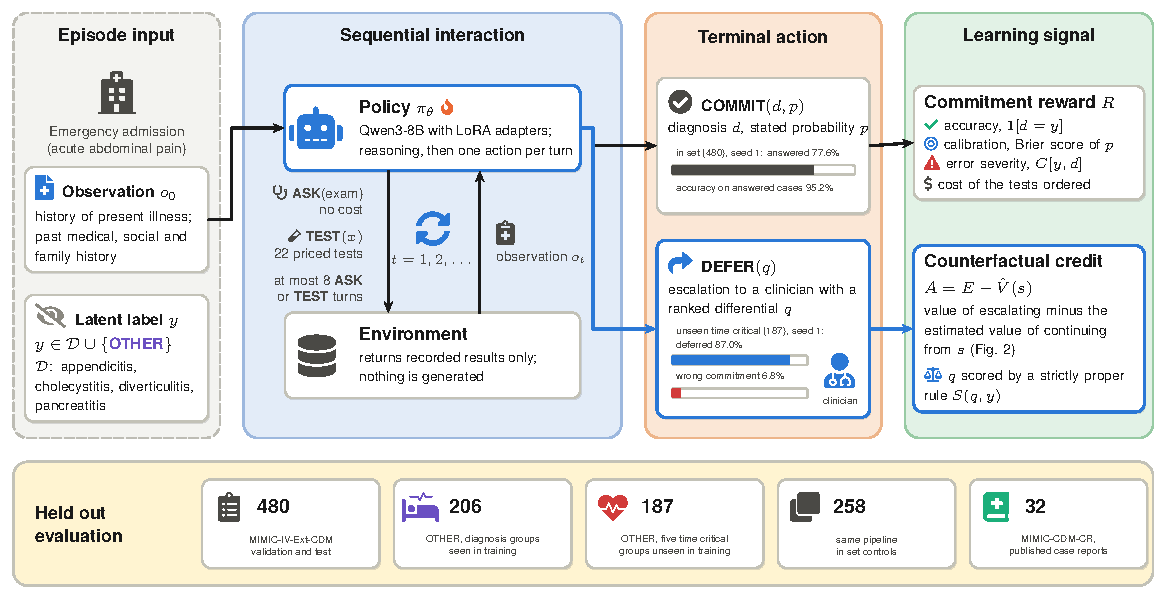
\includegraphics[width=\linewidth]{figures/fig_overview.pdf}
\caption{DEFER-Dx. One admission per episode. The agent sees the history at presentation and, each turn, asks for the examination, orders one of 22 priced tests, commits to a diagnosis with a stated probability, or defers to a clinician with a ranked differential. The label space is open: the four MIMIC-CDM conditions or OTHER. Commitments are scored in clinical units; deferrals are credited against the counterfactual of continuing (Figure~\ref{fig:cev}). Bars in the terminal action panel are measured results of DEFER-Dx (first seed; Table~\ref{tab:main}); the strip lists the held out evaluation sets.}
\alttext{Flow diagram in five shaded panels. An emergency admission with an observed history and a latent label feeds a policy, which loops with the environment by asking for the examination or ordering tests and receiving observations. The agent ends with either COMMIT, shown with a bar for the measured share of held out in set cases answered (77.6 percent, at 95.2 percent accuracy), or DEFER, shown with bars for the measured share of unseen time critical cases deferred (87.0 percent) and wrongly committed (6.8 percent), next to a clinician icon. COMMIT leads to a reward scored on accuracy, Brier score, error severity and test price; DEFER leads to a counterfactual credit. A strip at the bottom lists five evaluation sets with their sizes: 480, 206, 187, 258 and 32.}
\label{fig:overview}
\end{figure}

\subsection*{The counterfactual escalation value}
When an episode ends with a deferral at state $s$, the environment is rebuilt by deterministic replay and $K = 3$ continuations are sampled from $s$ with escalation disabled: a deferral is executed as a commitment to the top of its differential, and further tests remain allowed (Figure~\ref{fig:cev}a). Their mean return $\hat V(s)$, charging only tests ordered after $s$, values not escalating. The escalation itself is valued $E = V_\tau + \eta\,S(q, y) - \mu - \nu$, where $V_\tau$ is the reward of a calibrated decision that succeeds with probability $\tau$ (the clinician the credit assumes; annealed from 0.95 to 0.85), $S$ is the normalised multiclass Brier score of the handed over differential (strictly proper; $\eta = 0.3$), $\mu = 0.1$ is a handoff cost and $\nu$ is the price of a deferral set by the coverage controller. The deferral turn receives the advantage $A = E - \hat V(s)$; all other turns keep the group relative advantage. When the continuations would have settled the case, $A < 0$ and the agent learns to investigate; when they err even after testing, or the case is OTHER, $A > 0$ and the escalation is credited.

\begin{figure}[t]
\centering
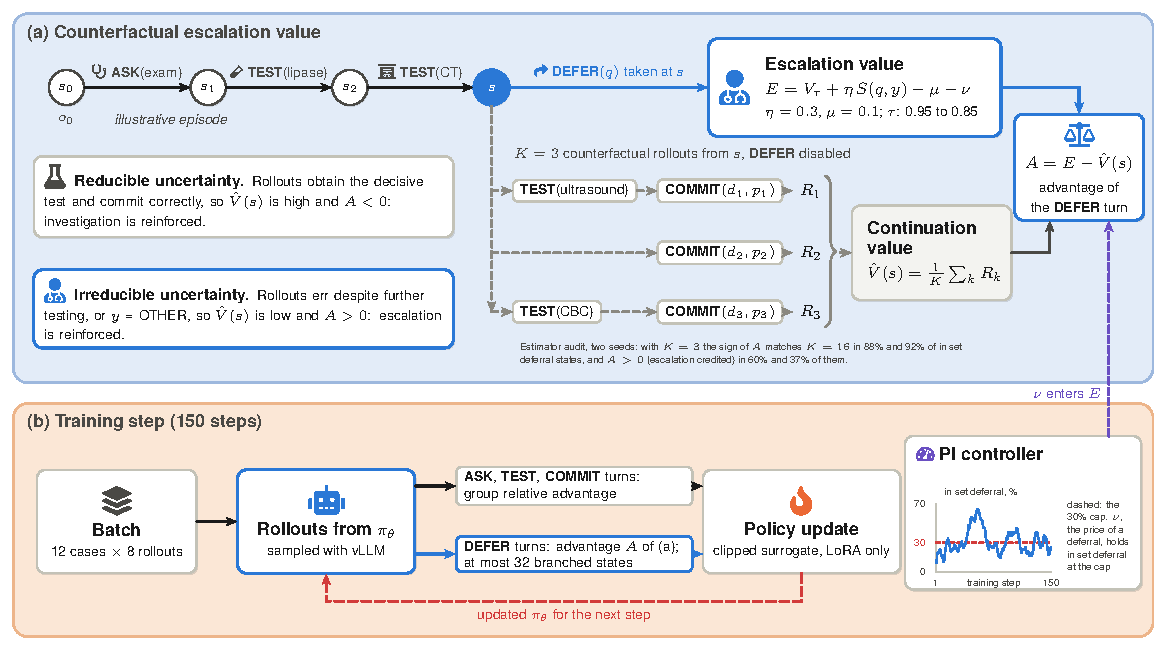
\includegraphics[width=\linewidth]{figures/fig_cev.pdf}
\caption{The counterfactual escalation value and one training step. (a) When an episode ends with DEFER at state $s$, the environment is replayed to $s$ and $K = 3$ forced continuations are sampled with escalation disabled. Their mean clinical return $\hat V(s)$ values not escalating; the DEFER turn's credit is $A = E - \hat V(s)$, where $E$ values the escalation, including a strictly proper score of the handoff. (b) Each step samples 12 cases with 8 episodes each, combines group relative advantages for ordinary turns with the escalation credit for DEFER turns, and updates the LoRA adapters; a PI controller holds in set deferral at a 30\% cap by setting $\nu$, the price of a deferral. The episode in (a) is illustrative. The controller inset shows DEFER-Dx's measured in set deferral in training batches (five step mean), and the audit figures under the rollouts are measured (Supplementary Figure S6).}
\alttext{Two stacked panels. Panel a shows a chain of states from s0 to s connected by ASK and TEST actions; from s a blue DEFER arrow leads to an escalation value box with the formula for E and its constants, while three dashed branches below run counterfactual rollouts that order tests and commit, giving returns R1 to R3 that are averaged into a continuation value box. Both boxes feed the advantage of the DEFER turn, A equals E minus V hat of s. Two callouts explain reducible uncertainty, where A is negative, and irreducible uncertainty, where A is positive. Panel b shows a training loop: batch, rollouts, two kinds of advantage, policy update with a red dashed arrow back to rollouts, and a PI controller panel plotting the measured in set deferral rate over 150 training steps, which peaks at 64 percent around step 55 and then stays near the dashed 30 percent cap (mean 28.6 percent over steps 101 to 150), with nu sent up into the escalation value.}
\label{fig:cev}
\end{figure}

\subsection*{Training and comparators}
Qwen3-8B\cite{qwen3} in thinking mode was fine tuned with LoRA adapters\cite{lora} (rank 16) by multiturn group relative policy optimisation\cite{grpo} on batches of 12 cases with 8 episodes each for 150 steps, with generation in vLLM\cite{vllm} on one 48 GB GPU. A PI controller on $\nu$ held in set deferral at or below 30\%; plain dual ascent wound up and cycled (Supplementary Figure S8). Comparators, all from the same base model and evaluated on the same cases: an identically trained agent without DEFER (the GRPO control, two seeds); the case level group consensus reward of prior work\cite{tiar,karl,awarl}, $\gamma(\tau - \hat p) - \mu$ with $\hat p$ the share of correct commitments in the episode group; and zero shot Qwen3-8B with forced choice or with deferral offered in the prompt. Second seeds changed only the seed. Each forced choice system was thresholded on its stated probability at DEFER-Dx's coverage, fitted on validation and applied to test and vice versa. Because stated probabilities are coarse (one value covers 14\% to 17\% of the control's cases), commitments tied at the cut were kept with a probability fitted to reach the target coverage, decided by a fixed hash of case and evaluation seed. We also evaluated selective risk thresholds\cite{geifman2017}, self consistency over three samples, and a learning to defer rule that defers whenever the stated probability is below the clinician's accuracy\cite{mozannar2020,madras2018,dvijotham2023}.

\subsection*{The receiving clinician}
For an escalated case (a deferral, or a commitment to OTHER, which names no diagnosis to act on), the clinician adopts the handoff's top suggestion with probability $f$ and otherwise decides correctly with probability 0.89, the accuracy of the MIMIC-CDM physicians\cite{hager2024} (Figure~\ref{fig:team}). We varied $f$ from 0 to 0.5; $f = 0.47$ is the excess of harmful decisions under misdirecting AI measured by Barrit and colleagues\cite{barrit2026}. Complicated disease was labelled from admission ICD codes and admission laboratory values by the guideline for each condition\cite{wses2020app,wses2020div,atlanta2012,tokyo2018} (Supplementary Methods).

\subsection*{Statistics}
Each number has a 95\% case level bootstrap interval (2,000 resamples, all evaluation seeds of a case resampled together); comparisons are paired bootstraps on the same cases. Pooled seed comparisons resample cases with training runs held fixed. Four primary tests were fixed before the second training seeds were run: pooled accuracy on answered cases and pooled unflagged errors against the thresholded control, and wrong commitments on never seen time critical cases against the consensus reward for each DEFER-Dx seed. Holm correction was applied within these four and, separately, across all 251 paired tests in the report; all other comparisons are exploratory.

% =========================== results ===========================
\section*{Results}

\subsection*{Learned escalation without collapse}
On the 480 held out CDM admissions, DEFER-Dx answered 77.6\% (74.3 to 80.6) of cases at 95.2\% (93.4 to 96.8) accuracy, with 3.8 (2.4 to 5.1) unflagged errors (wrong commitments without escalation) per 100 cases, against 24.1 for zero shot forced choice and 9.1 with deferral in the prompt (Table~\ref{tab:main}). Its stated probabilities were calibrated (ECE 0.042; Brier 0.047, the lowest of all systems). The second seed answered 73.2\% at 95.3\% accuracy with 3.5 unflagged errors per 100. Deferral did not collapse: the controller held in set deferral at its cap without the cycle of plain dual ascent.

\begin{table}[t]
\caption{Held out CDM admissions (480 cases, three evaluation seeds) and never seen time critical OTHER admissions (187). Thresholds are cross fitted at the first DEFER-Dx seed's coverage (78\%). Brackets: 95\% bootstrap intervals.}\label{tab:main}
\footnotesize
\begin{tabular}{@{}>{\RaggedRight}p{3.3cm}>{\centering}p{1.2cm}>{\centering}p{2.75cm}>{\centering}p{2.55cm}>{\centering}p{1.0cm}>{\centering}p{1.55cm}>{\centering\arraybackslash}p{1.15cm}@{}}
\toprule
System & Coverage, \% & Accuracy on answered, \% & Unflagged errors per 100 & Brier & Time critical wrong, \% & Tests per case \tabularnewline
\midrule
Zero shot, forced choice & 98.4 & 75.5 (72.2 to 78.6) & 24.1 (21.0 to 27.4) & 0.165 & 17.6 & 1.93 \tabularnewline
\quad with threshold & 77.2 & 82.8 (79.8 to 85.7) & 13.3 (11.0 to 15.6) & 0.136 & 11.1 & 1.93 \tabularnewline
Zero shot, DEFER in the prompt & 75.1 & 87.9 (85.2 to 90.4) & 9.1 (7.2 to 11.1) & 0.102 & 14.4 & 1.92 \tabularnewline
GRPO control, no DEFER & 93.8 & 87.8 (85.2 to 90.3) & 11.5 (9.1 to 13.9) & 0.091 & 15.0 & 1.48 \tabularnewline
\quad with threshold & 77.7 & 92.9 (90.7 to 94.9) & 5.6 (4.0 to 7.2) & 0.061 & 7.5 & 1.48 \tabularnewline
\quad second seed, with threshold & 77.6 & 89.9 (87.4 to 92.3) & 7.8 (6.0 to 9.7) & 0.087 & 9.8 & 2.18 \tabularnewline
Group consensus reward\cite{tiar,karl,awarl} & 82.6 & 94.0 (92.0 to 95.9) & 4.9 (3.4 to 6.6) & 0.055 & 11.4 & 1.83 \tabularnewline
\textbf{DEFER-Dx} & 77.6 & \textbf{95.2} (93.4 to 96.8) & 3.8 (2.4 to 5.1) & \textbf{0.047} & \textbf{6.8} & 0.84 \tabularnewline
\textbf{DEFER-Dx, second seed} & 73.2 & \textbf{95.3} (93.2 to 97.1) & \textbf{3.5} (2.2 to 5.0) & 0.048 & 7.1 & 0.89 \tabularnewline
\bottomrule
\end{tabular}
\end{table}

\subsection*{Learned versus post hoc deferral}
The fair comparison for learned deferral is a threshold on an identically trained agent\cite{che2026}. DEFER-Dx was more accurate on answered cases in all four pairings of two DEFER-Dx seeds with two control seeds (Figure~\ref{fig:seeds}): +2.3 (0.1 to 4.6), +5.3 (3.0 to 7.7), +1.1 ($-$0.8 to 3.3) and +4.1 (1.9 to 6.5) points. Pooled, the difference was +3.2 points (1.6 to 5.1), with 2.4 fewer unflagged errors per 100 (1.1 to 3.9) and a lower area under the risk coverage curve ($-$0.014, $-$0.031 to $-$0.005); DEFER-Dx's calibration error was higher (ECE +0.036). Without the tie rule, a plain cut overshot the target coverage and overstated the advantage (+3.1 instead of +2.3 for the first pairing). The margin depended mainly on the control's seed: identically trained controls differed in how well their confidence ranked their own errors (AURC 0.044 and 0.074), whereas DEFER-Dx's accuracy on answered cases was the same in both seeds. All four primary tests held after Holm correction within their family ($p \le 0.02$); across all 251 paired tests, the pooled accuracy difference had Holm $p = 0.060$ and the unflagged error difference 0.088.

\begin{figure}[t]
\centering
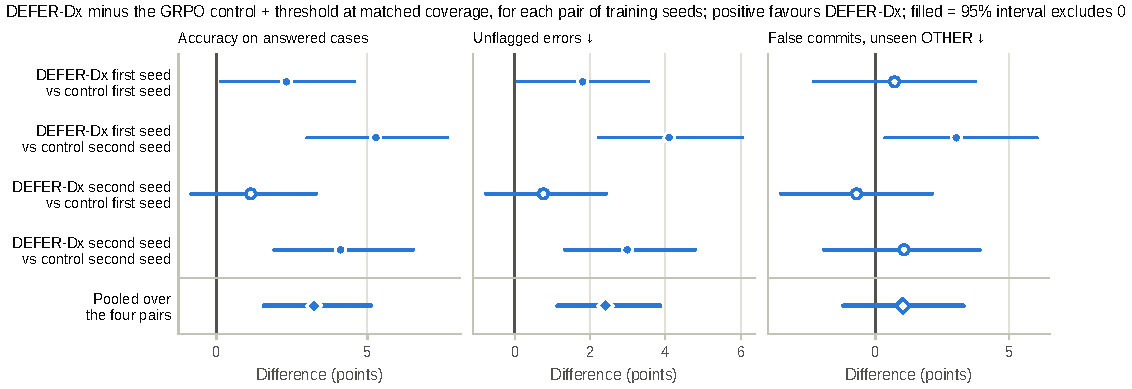
\includegraphics[width=\linewidth]{figures/fig_seed_pairings.pdf}
\caption{Learned versus post hoc deferral across training seeds. Each row compares one DEFER-Dx seed with one seed of the identically trained GRPO control, thresholded at that DEFER-Dx seed's coverage (paired, same 480 cases). The last row pools the four pairs with training runs held fixed. Positive values favour DEFER-Dx; filled markers have a 95\% interval that excludes 0.}
\alttext{Forest plot with five rows, four seed pairings and a pooled row, showing differences in accuracy on answered cases and in unflagged errors with 95 percent intervals. All four pairings favour DEFER-Dx; three of the four accuracy intervals exclude zero, and the pooled difference is plus 3.2 points.}
\label{fig:seeds}
\end{figure}

\subsection*{Unfamiliar, time critical presentations}
On 187 admissions from the five held out time critical groups, both DEFER-Dx seeds escalated 87.0\% of cases and committed to one of the four conditions in 6.8\% (4.3 to 10.0) and 7.1\% (4.3 to 10.3) (Figure~\ref{fig:openworld}), against 11.4\% for the consensus reward (differences $-$4.6, $-$8.0 to $-$1.4, and $-$4.3, $-$7.7 to $-$1.1), at the same accuracy on answered in set cases. On 206 OTHER admissions from groups seen in training the differences were $-$7.0 and $-$6.6 points. The thresholded control committed wrongly about as rarely (7.5\%) but differently: it escalated 21.0\% and committed to ``none of the four'' in 64.3\%. On 258 same pipeline in set controls DEFER-Dx named OTHER for 0.3\%, so its open world behaviour is not a source shortcut.

\begin{figure}[t]
\centering
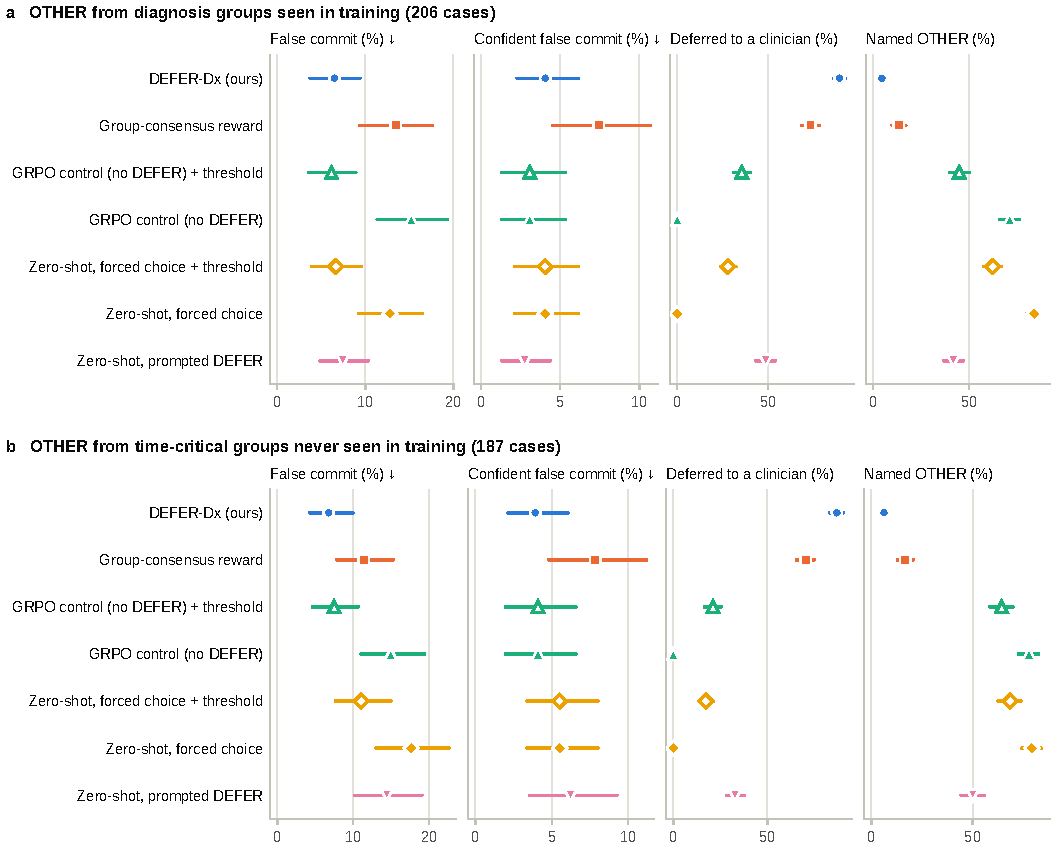
\includegraphics[width=\linewidth]{figures/fig_open_world.pdf}
\caption{Open world. Outcomes on OTHER admissions from (a) diagnosis groups seen in training and (b) five time critical groups never seen in training: wrong commitment to one of the four conditions, deferral, and naming OTHER. 95\% case level bootstrap intervals.}
\alttext{Grouped bar charts for two sets of OTHER admissions, comparing systems on the rate of wrong commitments, deferral and naming OTHER. Both DEFER-Dx seeds have the lowest wrong commitment rates among trained deferral rewards on never seen time critical cases, about 7 percent against 11 percent for the consensus reward.}
\label{fig:openworld}
\end{figure}

\subsection*{Complicated disease}
114 of 480 in set cases were complicated by guideline grade. A confidence threshold escalated complicated disease less often than uncomplicated disease (16.7\% vs 24.0\%; $-$7.4, $-$14.1 to $-$0.5), because complicated presentations produce confident commitments. DEFER-Dx did not (23.7\% vs 22.0\%), and at matched coverage it escalated complicated disease more than the thresholded control in all four seed pairings (+4.4 to +7.0 points). No system escalated complicated disease preferentially (Supplementary Figure S5).

\subsection*{What the handoff says, and the clinician who reads it}
The handoff's content depended on the training seed. 68.4\% of the first seed's in set handoffs ranked OTHER first, against 4.2\% for the second seed and 8.6\% for the consensus reward. On never seen time critical cases the pattern reversed: the first seed's handoffs suggested an in scope diagnosis in 21\%, the second seed's in 84\%. With an independent clinician ($f = 0$) every system's team accuracy on in set cases was about 94\% (Figure~\ref{fig:team}). At $f = 0.47$ the first seed's team accuracy fell to 86.8\%, against 91.5\% for the thresholded control ($-$4.7, $-$6.6 to $-$2.8), whereas the second seed's held (91.4\%); but on never seen time critical cases the second seed's handoffs led to wrong in scope diagnoses in 37.0\%, against 11.0\% for the thresholded control and 25.9\% for the consensus reward. The learning to defer rule was the safest on these terms (8.4\%), at almost twice the clinician workload (43\% of in set cases escalated, against 23\%).

\begin{figure}[t]
\centering
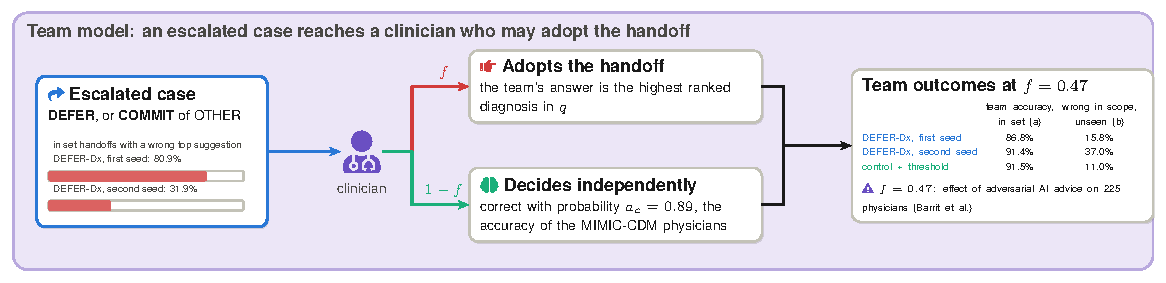
\includegraphics[width=\linewidth]{figures/fig_clinician.pdf}\\[4pt]
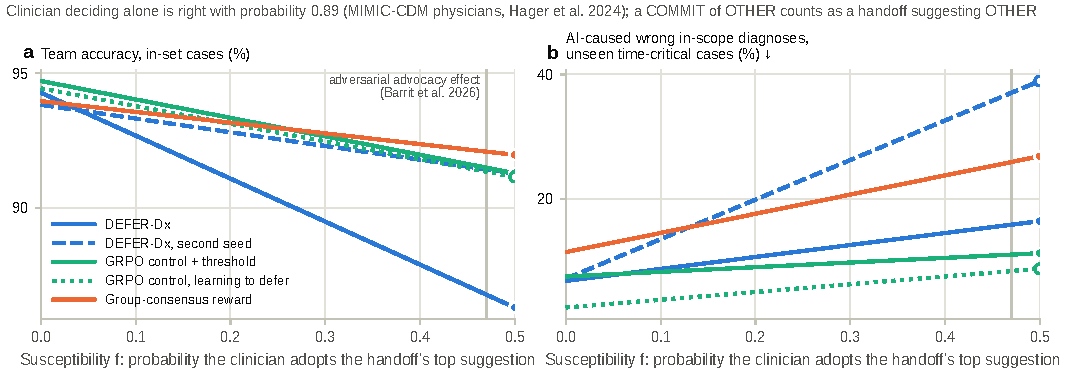
\includegraphics[width=\linewidth]{figures/fig_team.pdf}
\caption{The clinician who receives the handoff. Top: the team model; with probability $f$ the clinician adopts the handoff's top suggestion, otherwise decides independently with accuracy 0.89. Its bars and table are measured: the share of in set handoffs with a wrong top suggestion, and team outcomes at $f = 0.47$. (a) Team accuracy on in set cases. (b) Wrong in scope diagnoses caused by the AI on never seen time critical cases (its own wrong commitments plus clinicians who adopt an in scope suggestion). The vertical line marks the adversarial advocacy effect measured by Barrit and colleagues\cite{barrit2026}.}
\alttext{A schematic on top shows an escalated case, with bars for the share of in set handoffs whose top suggestion is wrong (80.9 percent for the first DEFER-Dx seed, 31.9 percent for the second), passing to a clinician, who either adopts the top suggestion with probability f or decides independently with accuracy 0.89, leading to a table of team outcomes at f equal to 0.47. Below, two line charts plot team outcomes against f from 0 to 0.5. In the left chart all systems start near 94 percent team accuracy; the first DEFER-Dx seed falls to about 87 percent at f equal to 0.47 while others stay near 91 to 92 percent. In the right chart wrong in scope diagnoses rise with f, most steeply for the second DEFER-Dx seed, to about 37 percent, and least for the learning to defer rule.}
\label{fig:team}
\end{figure}

\subsection*{What drives the escalation credit}
Resampling 16 continuations from 160 deferral states per final policy, the three continuation estimate used in training gave the credit the same sign as 16 continuations in 88\% and 92\% of in set states. Had it been unable to defer, the first seed's policy would have been right in only 32\% of its in set deferral states and the second seed's in 67\%: the first seed's deferrals were better targeted, and 60\% of them were credited against 37\%. If the assumed clinician were right in 70\% rather than 85\% of cases, 46\% rather than 60\% of the first seed's deferrals would be credited. Ablations at 100 steps (Table~\ref{tab:ablations}) separated the parts. A constant deferral reward matched DEFER-Dx on accuracy but deferred less and rarely named OTHER in its handoffs (24.7\% vs 89.0\% of never seen time critical cases). Removing the handoff score made handoffs less informative ($-$6.5 points, 3.5 to 9.3) and increased false commitments on OTHER (9.5\% vs 6.3\%). Pricing tests is not why DEFER-Dx escalates early: without the test cost the agent ordered fewer tests per case (1.01 vs 1.57) but costlier ones (\$1,166 vs \$1,042), escalated less (coverage 78.2\% vs 68.1\%; $-$10.1, $-$13.3 to $-$7.0) at the same accuracy on answered cases, and handed over less informative differentials ($-$12.9 points, 9.1 to 16.8). Without the coverage cap, in set deferral in training rose to 95\% after step 50 and the final policy answered 3.0\% of cases: the credit ranks states by the value of not escalating, and the cap turns that ranking into a budget. Weighting the handoff score more heavily ($\eta = 1.0$) moved the agent along the trade off that separated the two seeds rather than improving both.

\begin{table}[t]
\caption{Ablations at 100 training steps against DEFER-Dx at step 100 (held out CDM admissions, two evaluation seeds; time critical: never seen time critical OTHER admissions).}\label{tab:ablations}
\footnotesize
\begin{tabular}{@{}>{\RaggedRight}p{3.4cm}>{\centering}p{1.2cm}>{\centering}p{1.6cm}>{\centering}p{1.4cm}>{\centering}p{1.5cm}>{\centering}p{1.1cm}>{\RaggedRight\arraybackslash}p{3.15cm}@{}}
\toprule
Training & Coverage, \% & Accuracy on answered, \% & Unflagged per 100 & Time critical wrong, \% & Tests per case & Main change \tabularnewline
\midrule
DEFER-Dx, step 100 & 68.1 & 94.5 & 3.8 & 10.2 & 1.57 & reference \tabularnewline
Constant deferral reward & 77.5 & 94.9 & 4.0 & 10.7 & 2.02 & handoffs rarely name OTHER \tabularnewline
No handoff score ($\eta = 0$) & 75.9 & 95.6 & 3.3 & 12.8 & 1.06 & less informative handoffs \tabularnewline
No test cost ($c = 0$) & 78.2 & 93.6 & 5.0 & 14.4 & 1.01 & less escalation, worse handoffs \tabularnewline
No coverage cap & 3.0 & 93.1 & 0.2 & 0.5 & 0.12 & escalates almost every case \tabularnewline
Handoff score $\eta = 1.0$ & 74.1 & 92.0 & 5.9 & 10.4 & 0.90 & trades in set for open world handoffs \tabularnewline
\bottomrule
\end{tabular}
\end{table}

\subsection*{Published case reports and robustness}
On the 32 published cases (Figure~\ref{fig:cr}), the second DEFER-Dx seed escalated all 19 out of scope cases. The first escalated 17 and committed to an in scope diagnosis on two reported diagnostic traps: a ruptured aortic aneurysm with migratory right iliac fossa pain and an Alvarado score of 9, and a heterotopic pregnancy with a viable intrauterine pregnancy on ultrasound. The thresholded control ordered tests until its budget ran out on five cases whose deciding test lies outside the catalogue. On in scope cases DEFER-Dx escalated complicated disease and never uncomplicated disease. With every sentence containing CDM's diagnosis mask removed, accuracy on answered cases changed by $-$1.0 points ($-$2.0 to 0.0). The pattern of recorded tests predicts the diagnosis (macro AUROC 0.879 from recorded flags alone), but DEFER-Dx received a ``not performed'' reply in only 12\% to 17\% of episodes and was less accurate after one (89.7\% vs 95.7\%), so there is no sign that it profits from test availability. For context, on LA-CDM's test split, counting handoffs through their top choice, DEFER-Dx reached 76.4\% (71.1 to 81.0) mean class accuracy and its second seed 85.2\% (80.8 to 89.3), against 86.9\% for zero shot Qwen3-8B restricted to the four labels; LA-CDM reports 81.3\% in its own closed world environment\cite{lacdm}. These are not head to head comparisons, and learned deferral trades some full coverage accuracy for safety. Escalation and unflagged errors did not differ systematically by sex, race, insurance or language; patients aged 80 or older were escalated more often (Supplementary Table S2).

\begin{figure}[t]
\centering
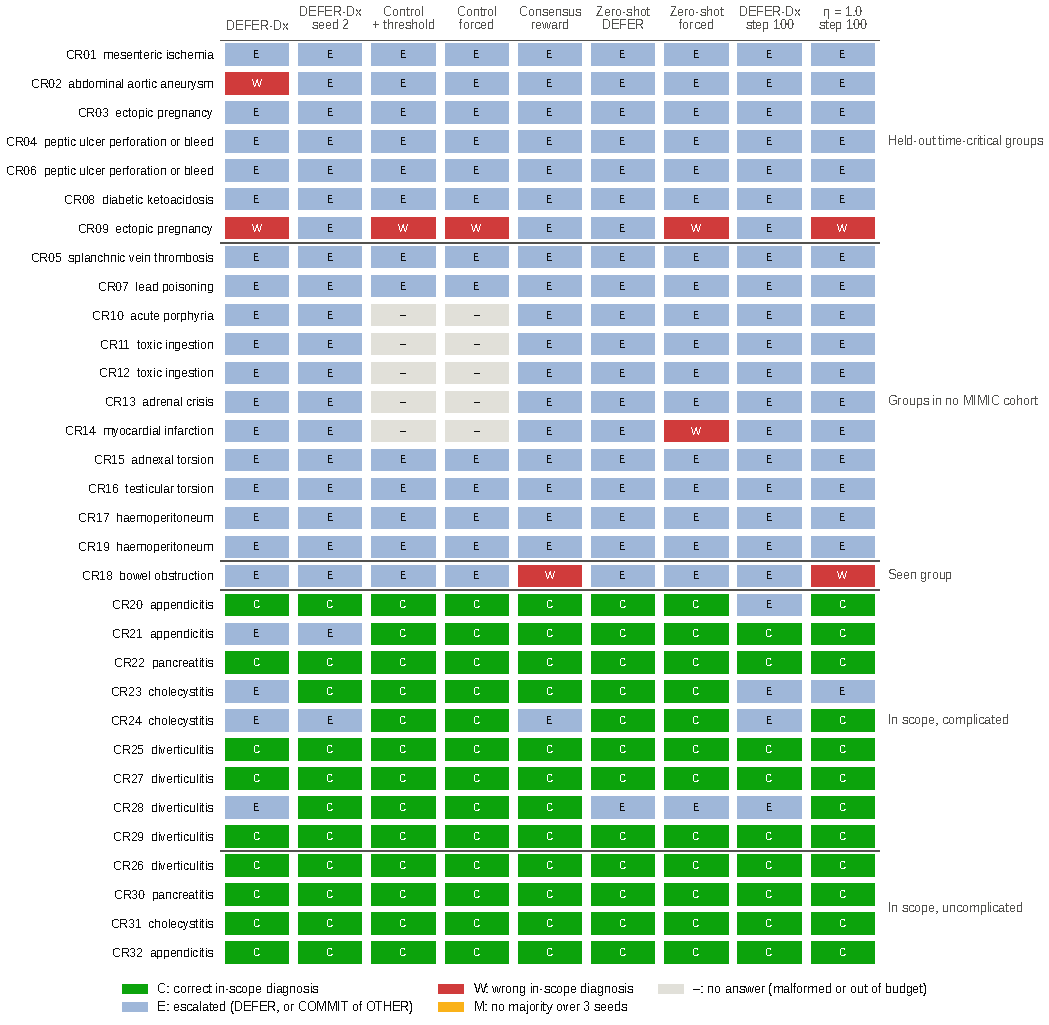
\includegraphics[width=\linewidth]{figures/fig_casereports.pdf}
\caption{MIMIC-CDM-CR: behaviour on 32 published case reports. Majority outcome over three evaluation seeds for each case (rows) and system (columns): C, correct in scope diagnosis; E, escalated; W, wrong in scope diagnosis; M, no majority. Rows are grouped by the held out time critical groups, groups in no MIMIC cohort, a group seen in training, and in scope cases with and without complications.}
\alttext{A grid with 32 rows of cases and one column per system, each cell a letter for the majority outcome. Out of scope rows are mostly E, escalated, for trained deferral systems; a few W cells mark wrong in scope diagnoses on reported diagnostic traps, and in scope rows are mostly C, correct.}
\label{fig:cr}
\end{figure}

% =========================== discussion ===========================
\section*{Discussion}

Learned deferral did not collapse. Crediting each escalation against what continuing from the same state would have achieved produced an agent that answered three quarters of in set cases at 95\% accuracy with fewer than four unflagged errors per 100, escalated 87\% of dangerous presentations it had never seen, and did both in two independent training runs. It outperformed the deferral reward of prior work on unfamiliar emergencies in both runs, and a threshold on an identically trained agent in all four seed pairings. How much it outperformed the threshold depended mainly on the threshold, because identically trained agents differed in how well their confidence ranked their own errors. Theory is right that a proper scored confidence makes thresholding a strong baseline\cite{che2026}; in our runs a learned operating point was the more reliable of the two. This complements informatics work that abstains after the fact\cite{swaminathan2024,brown2026}: when the model acts over several steps, the escalation can be credited where it happens.

The more important finding concerns the handoff. Deferral agents are evaluated as if the receiving clinician were independent of them, and under that assumption every system here reached the same team accuracy of about 94\%. Physicians are not independent of AI advice\cite{barrit2026,dratsch2023,goddard2012}. Once the clinician can be steered, the content of the handoff dominates: one run labelled uncertain in set cases ``none of the four'', the other escalated unfamiliar emergencies with an in scope suggestion, and either pattern would have cost patients under the susceptibility measured in physicians. A heavier proper score moved the agent between these patterns instead of fixing both. Regulatory guidance asks that clinicians be able to review the basis of a recommendation independently\cite{fda2026}; our results suggest that agents should be trained and evaluated against a clinician who might not.

Complicated disease is where a surgeon's decision matters most. A threshold sent it to the clinician less often than uncomplicated disease, because complicated presentations look certain; DEFER-Dx did not, but neither did it seek complicated disease out. A clinically useful agent would name the condition, grade it by the relevant guideline and escalate by grade\cite{nori2025}.

\textbf{Implications.} Learned deferral should be compared with a threshold on an identically trained model at exactly matched coverage, with more than one training run of each, since coarse confidences and seed to seed variation make unmatched or single run comparisons easy to misread. The volume of escalation should be set as a budget by the clinical service rather than left to the reward. Agents that defer should be evaluated in the open world, on external cases, and with a model of the clinician who receives the case, and the handoff should be trained against that clinician and assessed by clinicians.

\textbf{Limitations.} The data come from one centre and one organ system. OTHER labels are principal ICD codes; severity labels, the severity matrix and some test prices are proxies. The environment reveals only what was recorded, so test availability is informative, and it is static: the patient does not evolve while tests are pending. The clinician model is a sensitivity analysis calibrated to an adversarial study, not a measurement with these handoffs; a blinded rating of the handoffs and a user study are needed. Two training seeds per arm show seed to seed variation but cannot estimate it, and the consensus reward was evaluated with one seed (a second run was trained; its evaluation is pending). MIMIC-CDM-CR has 32 cases, too few for precise rates; it is an external check of behaviour, not a validation. No model here should be used for patient care.

\section*{Conclusion}
A counterfactual escalation value, used within a fixed escalation budget, trains a diagnostic agent whose deferral is stable, well targeted and more reliable than thresholding an identically trained agent. Whether that escalation is safe depends on the handoff, which should be trained and evaluated as carefully as the decision to escalate.

% =========================== statements ===========================
\section*{Funding}
[To be completed by the authors: funding sources, or ``This work received no specific funding.'']

\section*{Author contributions}
[CRediT roles for each author, entered at submission.]

\section*{Conflict of interest}
[To be completed by the authors.]

\section*{Ethics}
MIMIC-IV is deidentified and was used under the PhysioNet credentialed data use agreement. No MIMIC text was sent to a hosted model API: every model ran on local weights. Training and evaluation ran on the authors' own GPU, except one comparator training run (the consensus reward's second seed), which ran on a rented cloud GPU instance controlled by the authors; its data files were deleted with the instance. Published case reports were used under their open access licences, and MIMIC-CDM-CR contains no patient data beyond what the reports published.

\section*{Use of generative AI}
[Authors to confirm wording.] An AI assistant (Claude, Anthropic) was used to write and debug software, run analyses and draft text and figures. The authors reviewed, verified and take responsibility for all content. This is also disclosed in the cover letter.

\section*{Data availability}
Code, configurations, aggregate results, figures and MIMIC-CDM-CR are available at \url{https://github.com/GIND123/Clinical-Agent-Stanford}. MIMIC-IV, MIMIC-IV-Note and MIMIC-IV-Ext-CDM are available to credentialed users from PhysioNet; MIMIC-CDM-OW is rebuilt deterministically from them by the released code. Model weights trained on MIMIC will be released only through PhysioNet's credentialed channel.

\section*{Acknowledgments}
[To be completed by the authors.]

% =========================== references ===========================
\begin{thebibliography}{99}
\small
\bibitem{hager2024} Hager P, Jungmann F, Holland R, et al. Evaluation and mitigation of the limitations of large language models in clinical decision-making. \textit{Nat Med}. 2024;30:2613--2622. doi:10.1038/s41591-024-03097-1
\bibitem{johnson2023} Johnson AEW, Bulgarelli L, Shen L, et al. MIMIC-IV, a freely accessible electronic health record dataset. \textit{Sci Data}. 2023;10:1. doi:10.1038/s41597-022-01899-x
\bibitem{fda2026} US Food and Drug Administration. Clinical Decision Support Software: guidance for industry and Food and Drug Administration staff. Revised January 2026.
\bibitem{barrit2026} Barrit S, Salvagno M, Corriero A, et al. Subversion of clinical judgment by conversational artificial intelligence. \textit{medRxiv}. 2026. doi:10.64898/2026.10.05.26364541
\bibitem{goddard2012} Goddard K, Roudsari A, Wyatt JC. Automation bias: a systematic review of frequency, effect mediators, and mitigators. \textit{J Am Med Inform Assoc}. 2012;19:121--127. doi:10.1136/amiajnl-2011-000089
\bibitem{ldtl} Shen et al. LDTL. arXiv:2604.05116. 2026.
\bibitem{che2026} Che et al. Abstention as an action can kill both the reward gradient and the KL anchor. arXiv:2608.00301. 2026.
\bibitem{swaminathan2024} Swaminathan A, Lopez I, Wang W, et al. Selective prediction for extracting unstructured clinical data. \textit{J Am Med Inform Assoc}. 2024;31(1):188--197.
\bibitem{savage2025} Savage T, et al. Large language model uncertainty proxies: discrimination and calibration for medical diagnosis and treatment. \textit{J Am Med Inform Assoc}. 2025;32(1). doi:10.1093/jamia/ocae254
\bibitem{brown2026} Brown KE, Wrenn JO, Jackson NJ, et al. Auditor models to suppress poor artificial intelligence predictions can improve human-artificial intelligence collaborative performance. \textit{J Am Med Inform Assoc}. 2026;33(3):621--631. doi:10.1093/jamia/ocaf235
\bibitem{mozannar2020} Mozannar H, Sontag D. Consistent estimators for learning to defer to an expert. In: \textit{Proceedings of ICML}. 2020.
\bibitem{madras2018} Madras D, Pitassi T, Zemel R. Predict responsibly: improving fairness and accuracy by learning to defer. In: \textit{Advances in NeurIPS}. 2018.
\bibitem{dvijotham2023} Dvijotham KD, Winkens J, Barsbey M, et al. Enhancing the reliability and accuracy of AI-enabled diagnosis via complementarity-driven deferral to clinicians. \textit{Nat Med}. 2023;29:1814--1820. doi:10.1038/s41591-023-02437-x
\bibitem{tiar} Pan et al. TIAR. arXiv:2605.25850. 2026.
\bibitem{karl} Gao et al. KARL. arXiv:2604.22779. 2026.
\bibitem{awarl} Zhang et al. AWA-RL. arXiv:2607.10738. 2026.
\bibitem{trustmed} Zhan et al. TrustMed-RL. arXiv:2610.04387. 2026.
\bibitem{lacdm} Bani-Harouni et al. LA-CDM. In: \textit{Proceedings of ICLR}. 2026. arXiv:2506.13474.
\bibitem{qwen3} Yang A, et al. Qwen3 technical report. arXiv:2505.09388. 2025.
\bibitem{lora} Hu EJ, Shen Y, Wallis P, et al. LoRA: low-rank adaptation of large language models. In: \textit{Proceedings of ICLR}. 2022.
\bibitem{grpo} Shao Z, Wang P, Zhu Q, et al. DeepSeekMath: pushing the limits of mathematical reasoning in open language models. arXiv:2402.03300. 2024.
\bibitem{vllm} Kwon W, Li Z, Zhuang S, et al. Efficient memory management for large language model serving with PagedAttention. In: \textit{Proceedings of SOSP}. 2023.
\bibitem{geifman2017} Geifman Y, El-Yaniv R. Selective classification for deep neural networks. In: \textit{Advances in NeurIPS}. 2017.
\bibitem{wses2020app} Di Saverio S, Podda M, De Simone B, et al. Diagnosis and treatment of acute appendicitis: 2020 update of the WSES Jerusalem guidelines. \textit{World J Emerg Surg}. 2020;15:27. doi:10.1186/s13017-020-00306-3
\bibitem{wses2020div} Sartelli M, Weber DG, Kluger Y, et al. 2020 update of the WSES guidelines for the management of acute colonic diverticulitis in the emergency setting. \textit{World J Emerg Surg}. 2020;15:32. doi:10.1186/s13017-020-00313-4
\bibitem{atlanta2012} Banks PA, Bollen TL, Dervenis C, et al. Classification of acute pancreatitis 2012: revision of the Atlanta classification and definitions by international consensus. \textit{Gut}. 2013;62:102--111. doi:10.1136/gutjnl-2012-302779
\bibitem{tokyo2018} Yokoe M, Hata J, Takada T, et al. Tokyo Guidelines 2018: diagnostic criteria and severity grading of acute cholecystitis. \textit{J Hepatobiliary Pancreat Sci}. 2018;25:41--54. doi:10.1002/jhbp.515
\bibitem{dratsch2023} Dratsch T, Chen X, Rezazade Mehrizi M, et al. Automation bias in mammography: the impact of artificial intelligence BI-RADS suggestions on reader performance. \textit{Radiology}. 2023;307:e222176. doi:10.1148/radiol.222176
\bibitem{nori2025} Nori H, Daswani M, Kelly C, et al. Sequential diagnosis with language models. arXiv:2506.22405. 2025.
\end{thebibliography}

\end{document}
